\pdfminorversion 7
\pdfobjcompresslevel 3

\documentclass[a4paper]{article}
\special{papersize=210mm,297mm}
\usepackage[utf8]{inputenc}
\usepackage[T1]{fontenc}
\usepackage{cite}
\usepackage[francais]{babel}
\usepackage[bookmarks=false,colorlinks,linkcolor=blue]{hyperref}
\usepackage[top=3cm,bottom=2cm,left=3cm,right=2cm]{geometry}
\usepackage{graphicx}
\usepackage{wrapfig}
\usepackage{subfig}
\usepackage{eso-pic}
\usepackage{array}
\usepackage{color}
\usepackage[table]{xcolor}
\usepackage{url}
\usepackage{listings}
\usepackage{eurosym}
\usepackage{url}
\usepackage{textcomp}
\usepackage{fancyhdr} 

\definecolor{lightgray}{gray}{0.9}

\title{Rapport de Stage, Licence Informatique 3\up{ème} Année}
\author{Rémy \textsc{EL-SIBAIE BESOGNET}}

\newcommand{\HRule}{\rule{\linewidth}{0.5mm}}


\begin{document}


\begin{titlepage}

\begin{center}


% Upper part of the page

\textsc{\LARGE Université Paris Sud}\\[1.5cm]

\textsc{\Large Rapport de stage}\\[0.5cm]

\textsc{\Large Licence 3 Informatique}\\[0.5cm]

% Title
\HRule \\[0.4cm]
{ \huge \bfseries Ocaml et Combinatoire}\\[0.4cm]

\HRule \\[1.5cm]

% Author and supervisor
\begin{minipage}{0.4\textwidth}
\begin{flushleft} \large
\emph{Auteur:}\\
Rémy \textsc{EL SIBAÏE BESOGNET}
\end{flushleft}
\end{minipage}
\begin{minipage}{0.4\textwidth}
\begin{flushright} \large
\emph{Encadrant:} \\
Jean-Christophe \textsc{FILLIATRE}
\end{flushright}
\end{minipage}

\vfill

% Bottom of the page
{\large \today}

\end{center}

\end{titlepage}


~
\vfill

\begin{center}
\section*{Résumé}
\end{center}
En informatique, de nombreux problèmes de combinatoire tels que le problème des 
n-reines ou les problèmes de pavage de tuiles peuvent se formaliser d'une
façon commune :
La couverture exacte de matrice, soit EMC\footnote{Exact Matrix Covering}. 
Plusieurs algorithmes permettent alors 
de résoudre cette question et donc les problèmes ci-dessus de façon générique.

Dans ce travail, j'ai implémenté, en OCaml, deux algorithmes de
résolution du recouvrement exact de matrice ayant pour nom 
Zero-suppressed Binary Decision
Diagram et Dancing Links. 
Ensuite, j'ai apporté des méthodes 
simplifiant la modélisation des problèmes de combinatoire pour les ramener
à un probleme de type EMC. L'utilisateur peut par 
exemple utiliser un mini langage fourni pour décrire son problème. Pour finir, 
ce stage est une contribution au langage OCaml et 
en fera bénéficier sa communauté qui manquait cruellement d'outils de 
combinatoire dans les bibliothèques existantes.

\vfill




\newpage
\section*{Remerciements}

\newpage
\tableofcontents
\newpage
\listoffigures

\newpage
\section{Présentation}


J'ai effectué ce stage dans le cadre de ma troisième année de Licence en 
Informatique, sous la direction de Jean-Christophe Filliâtre (Equipe ProVal, 
LRI, Université Paris Sud 11 et CNRS / INRIA Saclay - Île-de-France). L'équipe 
ProVal a pour objectif de présenter des outils permettant de démontrer la 
validité de programmes par rapport à un comportement attendu en utilisant des
méthodes formelles de preuve.
Ces outils sont en majorité dévelopés en langage OCaml. 

Le but de mon stage n'est donc pas concentré sur le c\oe ur de métier de 
l'équipe. Il correspond plutôt à une contribution au langage OCaml. 
Cette contribution
prend la forme d'une bibliothèque OCaml pour la combinatoire, apportant
des méthodes simples permettant de modéliser des problèmes de combinatoire
sous forme de matrice de contraintes. Elle inclut l'implémentation de 
deux algorithmes permettant de résoudre le problème de la couverture exacte de
matrice ainsi qu'un langage pour décrire les problèmes de pavage.


\section{Couverture Exacte de Matrices}

\subsection{Définition}

Résoudre le problème de recouvrement exact de matrice 
(ou EMC~\footnote{Exact Matrix Covering en Anglais}) revient à,
partant d'une matrice de booléens donnée, trouver un sous-ensemble de 
lignes de cette matrice tel qu'il n'y ait qu'un et un seul '1' (ou \emph{true}) 
par colonne.
On considère par exemple la matrice suivante, de taille 4x5 avec les lignes
notées de '0' à '5' : 

\[
  \begin{array}{ c }
   0. \\
   1. \\
   2. \\
   3. \\
   4. \\
  \end{array}
\left(
  \begin{array}{ c c c c c }
   1 & 0 & 1 & 1 \\
   0 & 1 & 1 & 0 \\
   1 & 1 & 0 & 1 \\
   1 & 0 & 0 & 1 \\
   0 & 1 & 0 & 0
  \end{array} \right)
\]

Dans cette exemple, on vérifie que :

\begin{description}
\item[$ \{3, 4\} $] ne correspond pas à une solution du probleme (pas de 1 dans la 3\up{e} colonne)
\item[$ \{0, 4\} $] constitue bien une solution (un et un seul 1 par colonne)
\item[$ \{1, 3\} $] constitue une autre solution
\end{description}

Il faut comprendre que le problème EMC correspond en fait à une liste de 
contraintes. Le but est donc de choisir un ensemble de lignes qui satisfassent 
chaque contrainte une seule et une seule fois.
Ce problème est connu pour avoir une complexité importante. On pourra observer 
plus tard qu'il peut être résolu par \emph{backtracking}.


\subsection{Applications}

Résoudre EMC est finalement une forme de programmation par contrainte. 
Plusieurs problèmes peuvent donc être encodés dans EMC à 
condition de pouvoir les modéliser tels quels. Je donne ici quelques 
exemples.


\subsubsection{Pavage}
Un problème de pavage est la recherche du nombre de façon 
(ou d'au moins une façon) de recouvrir un
plateau de jeu avec des tuiles (c'est-à-dire des pièces) d'une taille et d'une
forme choisie. Ces problème s'encodent parfaitement dans un problème EMC
puisqu'on cherche généralement à recouvrir chaque case une seule et une 
seule fois. 
On prend le problème trivial suivant : \\


\emph{De combien de façon peut-on recouvrir un échiquier de taille 4x4 par 
des dominos ?}
\\

Ce problème est trivial puisqu'il existe une formule mathématique pour le 
résoudre. On en connaît donc facilement le nombre de solutions. 
Ici, on ne prend 
pas en compte la quantité de dominos que l'on peut poser ni les symétries 
éventuelles du problème. On construit alors la
matrice EMC correspondante. Une colonne de la matrice représente une case de 
l'échiquier et une ligne de cette même matrice représente une façon de poser 
une tuile. On numérote les cases de 0 à 15.

\begin{figure}[h]
\centering
\rowcolors{1}{lightgray}{lightgray}
\[
  \begin{array}{|c|c|c|c|}
		\hline
   	0 & 1 & 2 & 3 \\
		\hline
    4	& 5 & 6 & 7 \\
		\hline
   	8 & 9 & 10 & 11 \\
		\hline
   	12 & 13 & 14 & 15 \\
		\hline
\end{array}
	\textrm{ }
\begin{array}{ |c| }
	\hline
		\\
	\hline
    \\
	\hline
  \end{array}
	\textrm{ }
\begin{array}{ |c|c| }
	\hline
		& \\ 
	\hline
  \end{array}
\]
\caption{\label{chessboard4x4} Echiquier 4x4 et dominos}
\end{figure}

Par exemple, poser un domino horizontalement sur la case 0 donne la ligne
de matrice suivante : 

\[
  \begin{array}{ c c c c c c c c c c c c c c c c }
	1 & 1 & 0 & 0 & 0 & 0 & 0 & 0 & 0 & 0 & 0 & 0 & 0 & 0 & 0 & 0 
  \end{array}
\]

On continue l'opération pour chaque case et on ajoute la ligne correspondante
si la pièce peut être posée à cet endroit. 
Une fois que toutes les cases du plateau ont été testées pour chacune des pièces,
on obtient la matrice EMC résultat. On a bien modélisé un problème de pavage 
sous forme de problème EMC dont nous verrons les algorithmes de résolution par
la suite.

\subsubsection{Sudoku}

Il n'est pas indispensable de décrire à nouveau le principe du 
Sudoku~\cite{sudoku} qui est massivement connu. Mais une explication concernant
sa modélisation en EMC s'impose.
Pour les problèmes de pavage, la contrainte se situait au niveau des cases.Dans
le cas du Sudoku, mettre une valeur dans une case du quadrillage impose et
5 contraintes sur la valeur et l'espace : 
\begin{itemize}
\item la case (l'espace)
\item la ligne (la valeur)
\item la colonne (la valeur)
\item la cellule 3x3 (la valeur)
\end{itemize}


\begin{figure}[h]
\centering
\[
\begin{array}{|c|c|c||c|c|c||c|c|c|}
\hline
5 & 3 &   &   & 7 &   &  &   &    \\
\hline
6 &   &   & 1 & 9 & 5 &  &   &    \\
\hline
  & 9 & 8 &   &   &   &  & 6 &    \\
\hline
\hline
8 &   &   &   & 6 &   &   &   & 3 \\
\hline
4 &   &   & 8 &   & 3 &   &   & 1 \\
\hline
7 &   &   &   & 2 &   &   &   & 6 \\
\hline
\hline
  & 6 &   &   &   &   & 2 & 8 &   \\
\hline
  &   &   & 4 & 1 & 9 &   &   & 9 \\
\hline
  &   &   &   & 8 &   &   & 7 & 5 \\
\hline
\end{array}
\]
\caption{\label{sudoku} Sudoku exemple (source : \cite{sudoku})}
\end{figure}


Effectivement, une fois qu'un élément est mis dans une case, il utilise l'espace
de cette case et empêche n'importe quel élément de prendre sa position. 
Il empêche aussi qu'un élément de même \emph{valeur} soit mis dans 
sa colonne, sa ligne et sa cellule. 
Il faut donc représenter chacune de ces contraintes dans les lignes de 
la future matrice EMC. On calcule donc pour chaque contrainte, le nombre de
colonnes de EMC demandées. On va donc prendre cet exemple.


\begin{enumerate}
\item 81 cases dans un Sudoku
: 81 colonnes pour les cases
\item $ 9~\textrm{lignes} \times 9~\textrm{valeurs} = $ 
81 colonnes pour les lignes
\item $ 9~\textrm{colonnes} \times 9~\textrm{valeurs} = $ 
81 colonnes pour les colonnes
\item $ 9~\textrm{cellules} \times 9~\textrm{valeurs} = $
81 colonnes pour les cellules
\end{enumerate}

On obtient donc une matrice d'une largeur de $ 81 \times 4 = 324 $ colonnes. 
Dans notre exemple le cas où l'on ajoute un 4 à la 7\up{e} ligne, 8\up{e} 
colonne donnerait la ligne de matrice EMC représentée par le code OCaml 
suivant : 

\lstinputlisting[language=Caml]{../imports/setsudoku.ml}


\subsubsection{N-reines}

Les N-Reines (ou N-Queens) est un problème d'Informatique et de Mathématiques 
assez connu lui aussi. 
Le but est de placer \emph{n} reines d'échec sur un échiquier $ n \times n $ tel
qu'aucune de ces reines ne puisse attaquer une autre reine. On cherche,
dans notre cas, toutes les solutions.
La mise en place la plus connue est $ n = 8 $, où le nombre de solutions est 
92. 

On sent bien, ici aussi, que poser une reine sur l'échiquier dépend de
différentes contraintes. 

\begin{figure}[h]
\begin{center}
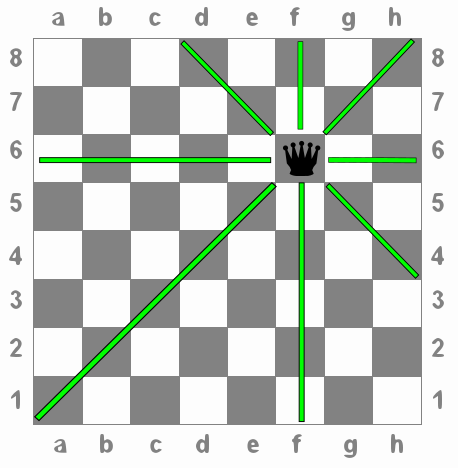
\includegraphics[height=0.2\textheight]{../imports/8queens.pdf}
\caption{\label{8queens} Poser une reine dans le problème des 8 reines}
\end{center}
\end{figure}

D'après la figure \ref{8queens}, on voit que les contraintes se font sur : 
\begin{itemize}
\item la ligne
\item la colonne
\item la diagonale gauche-droite
\item la diagonale droite-gauche
\end{itemize}

On peut éviter des considèrer les cases dans les contraintes : L'utilisation
d'une case est déjà comprise dans les quatres informations ci dessus (si une
reine une utilise une ligne et une colonne choisie, alors elle utilise
forcément une seule case).
De plus, au lieu d'avoir une matrice dont la largeur 
(le nombre de colonne de EMC) est
quadratique en la taille du problème, avec cette représentation, elle est
linéaire.

On a : 
\begin{enumerate}
\item 8 lignes
\item 8 colonnes
\item 15 diagonales gauche-droite
\item 15 diagonales droite-gauche
\end{enumerate}

Ce qui correspond à une matrice de 46 colonnes (et non 64 si on avait choisis
les cases comme contrainte).
Cette façon de représenter le problème des N-Queens en EMC vient de Knuth, qu'il
décrit dans son article Dancing~Links~\cite{dlx} (que l'on verra plus loin).

Par exemple, si on place une reine en (a,8) (voir figure \ref{8queens}), on 
génère alors la ligne de matrice EMC représentée par le code OCaml suivant : 

\lstinputlisting[language=Caml]{../imports/setqueens.ml}


\section{Recherche des solutions}

Aucun des algorithmes existant ne peuvent résoudre EMC
avec une complexité polynomiale. Les seules solutions connues ne sont en fait
que de la force brute, et c'est souvent le cas en combinatoire.
Ceci étant, les deux méthodes implémentées durant ce stage sont 
très malines et très élégantes. C'est sans surprise puisque leur auteur est 
Donald E. Knuth.
Chacun de ces algorithmes possède ses avantages et ses inconvénients qu'il faut 
exploiter.

\subsection{L'algorithme Dancing Links}

The Dancing links~\footnote{Les liens dansants} ou DLX~\cite{dlx} 
est une implémentation efficace de l'algorithme X de Donald 
E. Knuth, proposée par lui-même dans son article éponyme. 
L'algorithme X est une solution pour résoudre 
les problèmes de couverture exacte de matrice vu plus haut.



\subsubsection{Principe de base et structure de donnée}

Avant d'entrer dans le vif du sujet, il faut commencer par l'astuce autour de 
laquelle tourne l'algorithme Dancing Links.
Partons d'une structure connue : la liste doublement chaînée.
N'importe quel programmeur saura ajouter un élément dans une liste doublement
chaînée.


\begin{figure}[h]
\begin{center}
\includegraphics[scale=0.5]{../imports/add_elmt_dll.png}
\caption{\label{add_dll} Ajout d'un élément dans une liste doublement chaînée}
\end{center}
\end{figure}


Il suffit simplement de modifier quatres pointeurs comme indiqué 
figure~\ref{add_dll}. De même pour retirer un élément, il suffit de changer le 
pointeur de A vers C et le faire pointer vers B, et changer le pointeur de 
B vers C pour le faire pointer vers A. 

\begin{figure}[h]
\begin{center}
\includegraphics[scale=0.5]{../imports/delete.png}
\caption{\label{delete_dll} Suppression puis ré-ajout}
\end{center}
\end{figure}

On ne touche donc pas aux information de C. 
On peut donc connaître son ancienne position dans la liste. Si on veut
dans ce cas l'y remettre (Figure~\ref{delete_dll}), il suffit alors de modifier
à nouveau deux pointeurs
seulement : celui de Gauche[C] et celui de Droite[C] (donc de A et B).
Cette manipulation n'est pas courante mais elle convient parfaitement à 
l'algorithme X et elle est surtout très peu coûteuse.
Le nom poétique de cette algorithme vient de la manipulation astucieuse des 
pointeurs.

Maintenant que l'on connaît le principe, il faut comprendre pourquoi il est
utilisé. Avant de faire tourner l'algorithme, nous devons génerer une structure
de donnée adaptée à partir de la matrice EMC. Cette structure (exotique) 
est une matrice construite à partir de listes doublements
 chaînées, c'est à dire une \emph{matrice doublement chaînée} que l'on appellera 
 matrice DLX. Cette dernière ne relie que les valeurs \emph{true} ou '1' de
 la matrice EMC.

\begin{figure}[h]
\begin{center}$
\begin{array}{c c}
\left(\begin{array}{ c c c c c }
   1 & 1 \\
   0 & 1 
  \end{array}\right) &
\includegraphics[scale=0.4]{../imports/dlx_matrice.png}
\end{array}$
\caption{\label{fig:gen_dlx}Creation de la matrice DLX}
\end{center}
\end{figure}



Dans l'exemple~\ref{fig:gen_dlx}, on observe bien que seul les '1' sont représentés.
De plus, la matrice DLX contient un en-tête général \emph{h} duquel l'algorithme
démarre le parcourt ainsi qu'un en-tête par colonne.
Il faut évidemment bien faire attention au fait que la représentation est
cyclique et que le dernier élément d'une ligne pointe vers le premier et 
réciproquement (de même pour les colonnes).
On peut définir cette structure en langage OCaml de la façon suivante : 
	
\lstinputlisting[language=Caml]{../imports/node.ml}



\subsubsection{Déroulement}

Pour résumer le déroulement de façon simple, on parcourt les colonnes au fur et
à mesure et pour chaque colonne, on recouvre (retirer) cette colonne et chacune 
des lignes 
où la colonne comporte un '1'. Puis on recommence jusqu'à ce que la matrice 
soit vide. Ensuite on retourne en arrière pour le backtracking. On decouvre 
donc la dernière colonne couverte puis on recommence.

Et comme parfois, rien n'est plus explicite et clair qu'un morceau de OCaml, 
voici la fonction \emph{recherche} qui parcourt les solutions une par une et 
applique la fonction \emph{f} passée en paramètre :


\lstinputlisting[language=Caml]{../imports/search.ml}


\subsection{La structure Zero-Supressed Binary Decision Diagram}



Le ZSBDD, en français, Diagramme Binaire de décision sans zéro, ou 
plus simplement ZDD, est une structure de donnée qui découle de BDD (Binary 
Decision Diagram). BDD est utilisé pour décrire une fonction booléenne. Un
BDD correspond à un graphe orienté acyclique dont les feuilles ont pour valeur
\emph{true} et \emph{false}. Les n\oe uds ont chacun deux fils et contiennent 
des variables booléennes.

Le soucis de BDD dans les problèmes de combinatoire et que la majorité des 
champs finissent sur \emph{false} (ou $\bot$). C'est là qu'intervient le ZDD. 
qui a simplement une interprétation différente d'un BDD. Grâce au ZDD on 
supprime environ 40\% des n\oe uds.

\subsubsection{Definition et construction}



Basiquement un ZDD ressemble à un BDD avec quelques modifications : 

\begin{itemize}
\item Si un n\oe ud est une feuille alors sa valeur est $\bot$ ou $\top$
\item S'il est à droite et que c'est une feuille alors sa valeur est $\top$
\item Sinon, il est étiqueté par un entier i, avec comme sous arbre droit 
$A_1$ et sous arbre gauche $A_2$ et se note : i $\rightarrow$ $A_1$, $A_2$ tel
que $A_1$ et $A_2$ ne contiennent pas d'élément j avec j $\leq$ i \\
\end{itemize} 

Une façon simple d'imagine un ZDD est de le voir comme un ensemble d'ensemble 
d'entiers. 
On prend E = {0, 1,...,n}, $n \leq 1$. Un ZDD de E est une partie de l'ensemble 
des parties de E (soit un élément de P(P(E))). Il existe une transformation 
bijective qui permet de passer d'un ZDD à un ensemble et inversement.

On prend pour exemple le ZDD suivant : 

(les traits en poitillés représentent les fils gauches et les traits pleins les
fils droits.)
\begin{center}
\includegraphics[scale=0.4]{../imports/zdd_ex.pdf}
\end{center}

Moralement, l'arbre gauche représente les ensembles ne contenant 
pas la valeur
\emph{i} courante. L'arbre droit correspond aux ensembles qui
la contiennent.
L'ensemble représenté par un ZDD a autant d'élément que le ZDD a de feuilles 
dont la valeur est $\top$. On suppose que cet ensemble aura donc 4 élément.

Le moyen mnémotechnique pour vérifier des exemples triviaux est de parcourir 
l'arbre de bas en haut à partir des $\top$. On note un ensemble par $\top$.
Quand on passe d'un n\oe ud fils à un n\oe ud père, si le fils était à droite
on ajoute le père à l'ensemble en construction, sinon non. Une fois en haut
on recommence l'opération à partir d'une nouvelle feuille $\top$.

\begin{itemize}
\item Top tout à gauche : $\top$ à droite : 1 y est, 1 à gauche : 0 n'y est pas.
On obtient l'ensemble \{1\}
\item Top milieu gauche : $\top$ à droite : 2 y est, 2 à gauche : 1 n'y est pas,
1 à gauche : 0 n'y est pas. On obtient l'ensemble \{2\}
\item Top milieu droite : $\top$ à gauche : 1 n'y est pas, 1 à droite : 0 y est.
On obtient l'ensemble : \{0\}
\item Top tout à droite : $\top$ à droite : 2 y est, 2 à droite : 1 y est. 1 à
droite : 0 y est. On obtient l'ensemble \{0, 1, 2\}
\end{itemize}

Ce ZDD est donc l'ensemble : \{\{0, 1, 2\}, \{0\}, \{1\}, \{2\}\}

On peut aussi évidemment construire un ZDD à partir d'un ensemble.


\subsubsection{Une structure optimisée}

\subsubsection{Utilisation pour EMC}



\subsection{ZDD vs DLX}


\section{Une bibliothèque OCaml}

\subsection{Architecture}

\subsection{Un mini langage pour les problèmes de pavage}

 expliquer optimisation des symétries ici

\section{Conclusion}


\bibliographystyle{plain}
\bibliography{./biblio}


\end{document}
